\chapter{The \pkg{LiteBook} Template}

\section{The purpose of this package}
This template provides a fresh cover and chapter design for book. Welcome to feedback bugs or ideas via email \href{mailto:xiamyphys@gmail.com}{\ttfamily xiamyphys@gmail.com} or \href{https://github.com/xiamyphys/fadingimage}{GitHub}.

This template was originally used for the reformatting of the textbook \emph{General Relativity, R. Wald}, you can download it from \url{https://github.com/xiamyphys/LaTeX-General-Relativity-R.Wald}.

\section{Installing \pkg{LiteBook} and loading it}
For portable version, simply download latest \verb|litebook.cls| file from \href{https://github.com/xiamyphys/LiteBook}{GitHub} or \href{https://ctan.org/pkg/litebook}{CTAN} and save it under your working directory. This way of installation is simple and convenient, but you have to manually update \verb|.cls| now and then.

However, I strongly suggest that you should use terminal/cmd to implement the commands to update all the packages (and install this package) to the latest version or switch to portable version instead
\begin{verbatim}
    sudo tlmgr update --self --all
\end{verbatim}

If you are in some areas with awful Internet environment (such as a), you can choose proper mirror source or use other means\footnote{Please comply with local network regulations.}. To learn more, please refer to \href{https://tex.stackexchange.com/questions/55437/how-do-i-update-my-tex-distribution}{How do I update my \textsf{\TeX} distribution?}

\section{Compatibility}
The test environments are macOS + Mac\TeX{} 2024 / Overleaf and they all work fine for \hologo{pdfLaTeX} and \hologo{XeLaTeX} compilers, Windows, Linux and Unix platforms compatibility unknown.

\section{Cover Information Settings}
Just like the cover of this document, there are 5 lines of information on the cover and a cover image, the corresponding commands are

\begin{verbatim}
    \title{The \pkg{LiteBook} Template}     \subtitle{Version 0.1a \today}
    \press{The University of Chicago Press} \author{Hsia Mingyu}
    \bioinfo{Hangzhou Dianzi University}    \cover{Beautiful-realities.jpeg}
\end{verbatim}

Here, the same as the \pkg{book} class, the command \cmd{title} could not be omitted, or it will return an error, and there will be a warning if the command \cmd{author} is omitted.

\section{Preset packages and commands}
This package has been preset with the following packages: 
\begin{table}[!ht]
    \centering
    \begin{tabular}{l l l l l l}
        \toprule
        \pkg{amsmath} & \pkg{amssymb} & \pkg{mathrsfs} & \pkg{esvect} & \pkg{physics2,fixdif} & \pkg{bm}\\
        \midrule
        \pkg{derivative} & \pkg{cancel} & \pkg{extarrows} & \pkg{siunitx} & \pkg{nicefrac} & \pkg{nicematrix}\\
        \midrule
        \pkg{booktabs} & \pkg{tabularx} & \pkg{diagbox} & \pkg{multicol} & \pkg{multirow} & \pkg{refstyle}\\
        \bottomrule
    \end{tabular}
\end{table}

You can click on them to go to the homepage to view the documentation.

And commands \verb|\i|, \verb|\e|, \verb|\T| has been defined to input 
$\i$, $\e$ in roman (non-italic) text and matrix transpose symbol $\T$, which can help you typeset math quickly.

The template has been preset the following reference command with the \pkg{refstyle} package: \verb|\eqref{#1}|, \verb|\figref{#1}| and \verb|tabref{#1}|, you can add other commands like these with the \pkg{refstyle} package.

\section{Preset Environments}
The template has been preset the following envrionments with the \pkg{amsthm} package

\begin{tcblisting}{sidebyside}
    \begin{theorem}
        A theorem environment.
    \end{theorem}
\end{tcblisting}

\begin{tcblisting}{sidebyside}
    \begin{example}
        An example environment.
    \end{example}
\end{tcblisting}

\begin{tcblisting}{sidebyside}
    \begin{problem}
        A problem environment.
    \end{problem}
\end{tcblisting}

\begin{tcblisting}{sidebyside}
    \begin{solution}
        A solution environment.
    \end{solution}
\end{tcblisting}

You can add other envrionments like these with the \pkg{amsthm} package.

\section{Equation Test}
\begin{equation}
    \ab(\frac1{c^2}\frac{\partial^2}{\partial t^2}-\nabla^2+\frac{mc^2}{\hbar^2})\psi(\mathbf x,t)=0
    \label{1.6.1}
\end{equation}

The Klein-Gordon \eqref{1.6.1}.

\section{Figure and Caption Side by Side Test}
\begin{figure}[!ht]
\begin{minipage}{.32\textwidth}
    \caption{A diagram showing the causal structure of spacetime in special relativity. The ``light cone'' of $p$ rather than a ``surface of simultaneity'' with $p$ now plays a fundamental role in determining the causal relationship of $p$ to other events.}
    \label{1.1}
\end{minipage}
\hfill
\begin{minipage}{.64\textwidth}
    \centering
    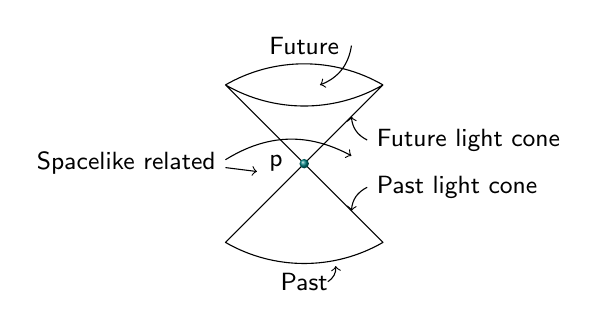
\begin{tikzpicture}
        \draw [line join=round,line cap=round] (-1,1) -- (1,-1) arc (-60:-120:2) -- (1,1) arc (-60:-120:2) arc (-60:-120:-2);
        \shade [ball color=teal] (0,0) circle (.06) node [anchor=east,xshift=-1ex] {\sffamily\small p};
        \node at (0,1.5) {\sffamily\small Future};
        \path [->] (.6,1.5) edge [bend left] (.2,1);
        \node at (0,-1.5) {\sffamily\small Past};
        \path [->] (.3,-1.5) edge [bend right] (.4,-1.3);
        \node [left] at (-1,0) {\sffamily\small Spacelike related};
        \path [->] (-1,-.05) edge (-.6,-.1);
        \path [->] (-1,.05) edge [bend left] (.6,.1);
        \node [right] at (.8,.3) {\sffamily\small Future light cone};
        \path [->] (.8,.3) edge [bend left] (.6,.6);
        \node [right] at (.8,-.3) {\sffamily\small Past light cone};
        \path [->] (.8,-.3) edge [bend right] (.6,-.6);
    \end{tikzpicture}
\end{minipage}
\end{figure}

\figref{1.1} shows the Light Cone.

\section{Warnings}

Due to the template has used the \pkg{FadingImage} package to add a fading image on the cover, when you use the \hologo{pdfLaTeX} compiler, should run it for two times or the cover image will not appear on the correct location, also, there will be a double question mark when referring to labels.


% amsthm